\subsection{Implementação do Módulo Evoluído}
\label{subsec:module_implementation}
Após elaborar a sequência de etapas que demonstrou performance promissora no pré-tramento dos dados coletados pelo dispositivo BIoT, e consequentemente um melhor reconhecimento de eventos de interesse, é necessário realizar a implementação da abordagem evoluída no contexto do sistema SAFE/UFRJ, para que seu funcionamento seja avaliado em conformidade com todo os subsistemas que compõem a aplicação IoT. Deste modo, a presente subseção pretende descrever todo o processo de evolução dos componentes de \textit{software}, bem como as decisões arquiteturais adotadas tendo em vista o ambiente de desenvolvimento embarcado, no qual sistemas de \textit{software} IoT se enquadram.

Atualmente, o dispositivo BIoT é composto por um microcontrolador ESP32 conectado há uma coletânea de sensores encarregados de coletar informações sobre a qualidade do ar interno e monitorar o fluxo de pessoas em uma instalação \cite{SAFE-IOT}. Para o desenvolvimento em embarcados, o uso de memória e processamento requer mais atenção, tendo em vista que este tipo de \textit{hardware} possui recursos mais limitados que estações de trabalho convencionais. O ESP32 pode ser considerado um microcontrolador poderoso, pois dispõe de um processador com dois núcleos, 520 Kbytes(KB) de memória SRAM(\textit{Static Random Acess Memory)}, 448KB de memória ROM(\textit{Read-only Memory} e 4 Megabytes(MB) destinados a memória Flash \cite{hercog_design_2023}. Além disso, esta placa de desenvolvimento apresenta módulos de Wi-Fi e Bluetooth de fábrica, facilitando a implementação de comunicação sem fio, um requisito para implementações IoT \cite{motta_evidence-based_2023}.

A arquitetura \textit{dual-core} do microcontrolador em uso, possibilitou que o \textit{software} desenvolvido para o BIoT, fosse implementado através de paradigmas de computação concorrente, como estratégias \textit{lock-free}, para a alocação dinâmica de memória e políticas de escalonamento de tarefas \cite{kim_lwmalloc_2025, lee_fast_2011}. Estas decisões arquiteturais foram mantidas durante a evolução do dispositivo. Deste modo, todas as funções implementadas, que configuram a evolução do BIoT, seguem as mesmas regras de modelagem e desenvolvimento, um exemplo é a Figura \ref{fig:get_ultrassonic_measures_workflow}, a qual apresenta a sequência de etapas que constituem a tarefa de coleta e armazenamento de medidas, todo este processo é executado por um núcleo arbitrário designado pelo escalonador de tarefas.

\begin{figure}[H]
    \centering
    \fbox{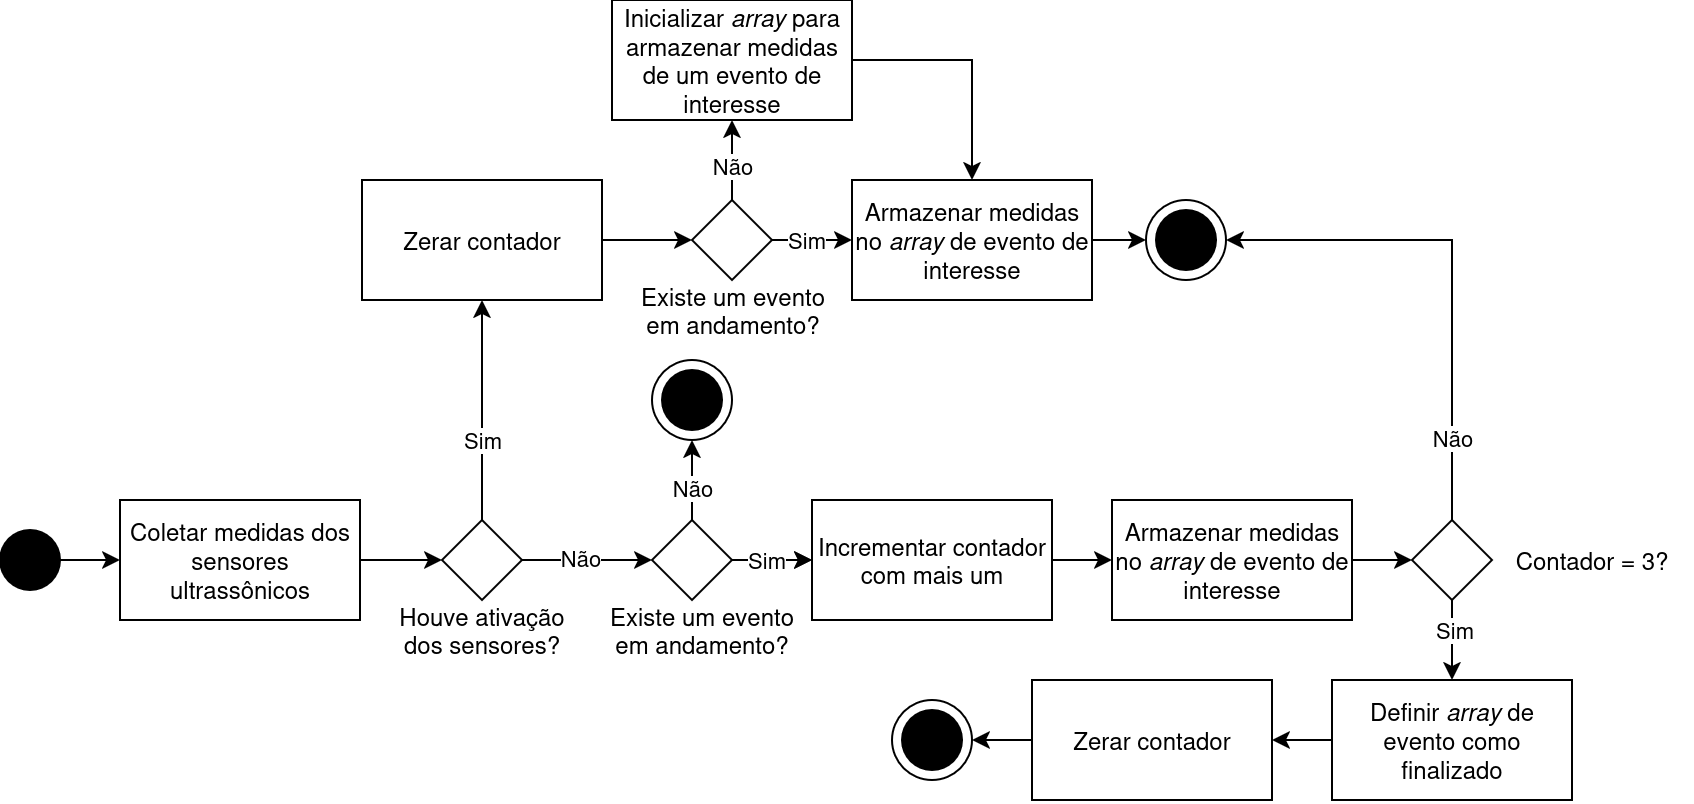
\includegraphics[width=\linewidth]{images/fluxograma_coleta_medidas_hcsr04.png}}
    \caption{Fluxo de construção de eventos de interesse}
    \label{fig:get_ultrassonic_measures_workflow}
\end{figure}

O processo de construir estruturas de dados, para armazenar medidas que compõem um possível evento de interesse, consiste nas primeiras duas etapas da estratégia de contagem de pessoas descrita previamente na Subseção \ref{subsec:module_evolution}. Entretanto, diferentemente do contexto de elaboração da abordagem, onde o \textit{dataset} submetido ao pré-tratamento é antecipadamente coletado, na circunstância da aplicação este conjunto de dados é construído de forma incremental e síncrona medida por dedida. O fluxograma presente na Figura \ref{fig:get_ultrassonic_measures_workflow} apresenta toda lógica de inclusão das medidas para composição de um evento. Em síntese, para cada ativação de um dos sensores, o dispositivo acumula medidas em um vetor até que sejam detectados três períodos consecutivos de inatividade, de acordo com as condições destacadas na subseção anterior, após isso o vetor recebe uma etiqueta que sinaliza para a tarefa em espera, que aquele grupo de dados está pronto para a próxima etapa, bem como pode conter um evento de interesse. 

\begin{figure}[H]
    \centering
    \fbox{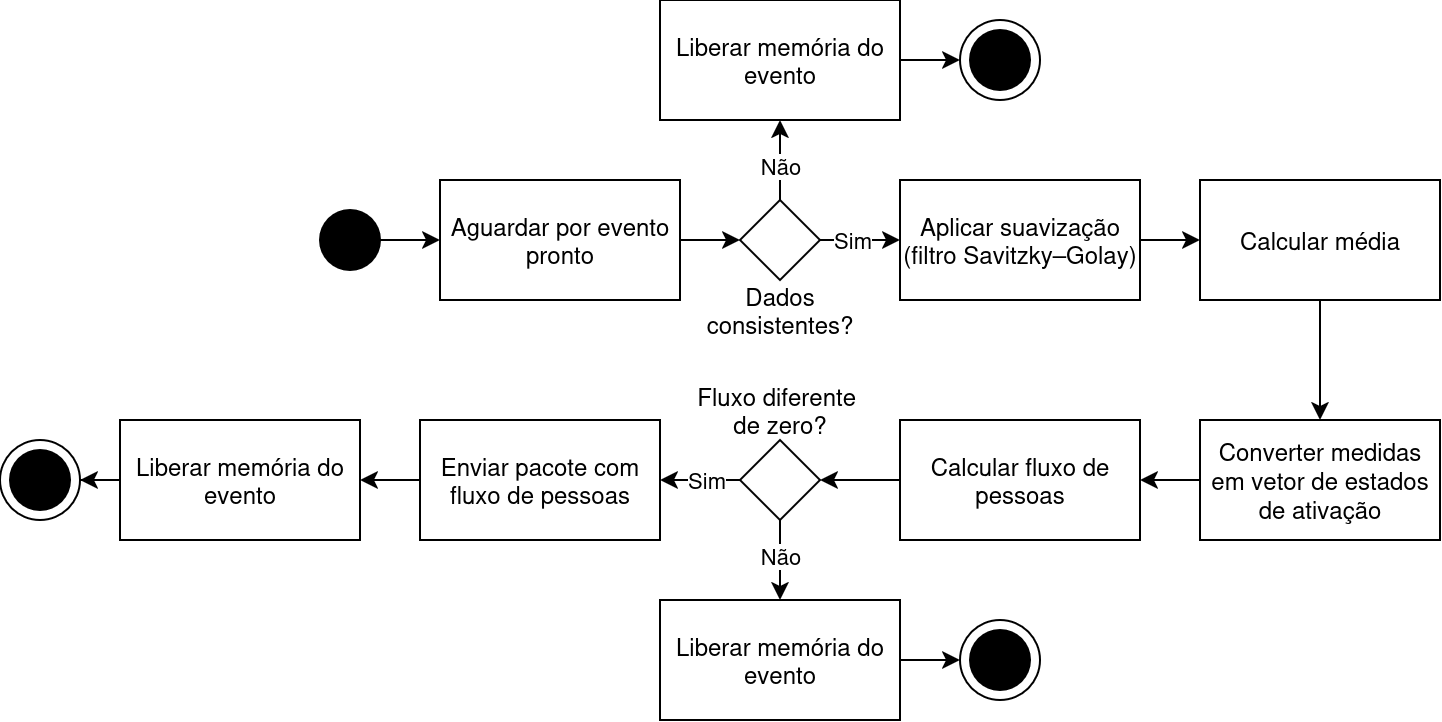
\includegraphics[width=\linewidth]{images/fluxograma_tarefa_consumo_eventos.png}}
    \caption{Sequência de atividades para calcular o fluxo de pessoas em eventos registrados}
    \label{fig:get_events_workflow}
\end{figure}

Após a atribuição do status de pronto ao evento, o vetor de medidas permanece em espera até que o escalonador execute o procedimento responsável pelo cálculo do fluxo de pessoas. A Figura \ref{fig:get_events_workflow} apresenta o fluxograma dessa tarefa, cujo objetivo é complementar as etapas da estratégia previamente descrita na Subseção \ref{subsec:module_evolution}. Assim, as atividades representadas correspondem majoritariamente a processos já detalhados, com exceção da liberação de memória associada à alocação dinâmica e do envio de pacotes, referentes à comunicação sem fio do dispositivo BIoT para publicação das medidas. Destaca-se ainda a etapa de suavização dos dados, implementada por meio de uma biblioteca adaptada exclusivamente para os requisitos do sistema. O Algoritmo \ref{alg:suavizacao_sg_nearest} descreve de forma mais rigorosa a lógica de funcionamento desse componente.

\begin{algorithm}[H]
\caption{Suavização Savitzky--Golay com bordas por vizinho mais próximo}
\label{alg:suavizacao_sg_nearest}
\begin{algorithmic}[1]
\Require vetor de entrada $x[0..L-1]$, vetor de saída $y[0..L-1]$, $L$, $janela$, $ordemPol$
\Ensure $y$ preenchido com a série suavizada, ou falha
\Function{SuavizarSG}{$x,y,L,janela,ordemPol$}

  \If{$x=\textsc{null}$ \textbf{or} $y=\textsc{null}$ \textbf{or} $L=0$}
    \State \Return \textbf{false} \Comment{Validação de ponteiros e tamanho}
  \EndIf

  \State $janela \gets \Call{AjustarJanela}{L,janela}$ \Comment{Força $3 \le janela \le 21$ e ímpar}
  \If{$janela < 3$ \textbf{or} $janela > 21$ \textbf{or} $janela$ é par}
    \State \Return \textbf{false} \Comment{Janela inválida após ajuste}
  \EndIf

  \State $ordemPol \gets \min(5,\max(2,ordemPol))$ \Comment{Limita a ordem polinomial em $[2,5]$}
  \If{$janela < 4$}
    \State $ordemPol \gets 2$ \Comment{Regra: janela muito curta força ordem 2}
  \EndIf

  \State $linha \gets (janela-3)/2$ \Comment{Mapeia janela (3..21) para linha na tabela}
  \State $coef \gets \begin{cases}
	  CoefSG_{P3}[\textit{linha}], & \text{se } ordemPol \le 3\\
	  CoefSG_{P5}[\textit{linha}], & \text{caso contrário}
  \end{cases}$ \Comment{Escolha da tabela de coeficientes}

  \State $M \gets \lfloor janela/2 \rfloor$ \Comment{Semi-janela: amostras em cada lado}
  \State $ultimo \gets L-1$ \Comment{Último índice válido}
  \State $denom \gets coef[0]$ \Comment{Denominador (normalização)}

  \For{$n \gets 0$ \textbf{to} $L-1$}
    \State $acum \gets coef[1+M]\cdot x[n]$ \Comment{Peso do centro ($k=0$)}
    \For{$k \gets 1$ \textbf{to} $M$}
      \State $h \gets coef[1+(M-k)]$ \Comment{Peso simétrico para distância $k$}
      \State $i_m \gets \Call{Limitar}{n-k,0,ultimo}$ \Comment{Borda: satura índice à esquerda}
      \State $i_p \gets \Call{Limitar}{n+k,0,ultimo}$ \Comment{Borda: satura índice à direita}
      \State $acum \gets acum + h\cdot (x[i_m] + x[i_p])$ \Comment{Soma par simétrico}
    \EndFor
    \State $y[n] \gets acum/denom$ \Comment{Normaliza e grava a saída}
  \EndFor

  \State \Return \textbf{true} \Comment{Suavização concluída}
\EndFunction
\end{algorithmic}
\end{algorithm}

A implementação do filtro de Savitsky-Golay foi realizada em conformidade com as equações X e Y previamente discutidas na subseção anterior. No entanto, o componente possui algumas particularidades devido ao contexto da aplicação, como restrições da ordem do polimônio e limites bem definidos para o tamanho da janela de suavização. A imposição deste tipo de restrição tem como objetivo, prevenir que o algoritmo adote configurações que podem impedir ou prejudicar a suavização dos dados e consequentemente o cálculo do fluxo de pessoas. Por fim, destaca-se que todas delimitações foram obtidas de forma experimental através dos estudos realizados durante a etapa de análise exploratória dos dados e avaliação da estratégia evoluída. 


Para realizar estas restrições duas funções foram implementadas, ``AjustarJanela'' e ``Limitar'', a primeira função tem como objetivo garantir que o tamanho da janela de suavização sempre esteja dentro do limite fechado $[3..21]$ e corresponda a um valor ímpar, esta última limitação é herdada da formulação matemática do filtro de SG e é necessária para que ele atue como o esperado. A segunda função, representa o método adotado para lidar com os valores que estão na borda do conjunto de medidas, como o filtro adotado realiza somas simétricas em torno da posição central ($n+k$ e $n-k$), nas regiões próximas ao início ou fim do vetor, estes índices podem se tornar negativos ou superiores ao tamanho do conjunto de medidas ($L-1$). A operação de saturação, impede que isso aconteça substituindo os valores fora do intervalo pelo índice válido mais próximo, esta estratégia é conhecida como tratamento de bordas por vizinho mais próximo (\textit{nearest boundary condition}). Este método foi adotado pois confere aos valores brutos inicias e finais maior impacto no cálculo de influência, isto é positivo para o desempenho da aplicação, pois normalmente estas medidas correspondem a variações de estado, logo devem ser percebidas de forma clara pelo algoritmo. 

Por fim, destaca-se, as principais implicações da evolução do dispositivo BIoT e as consequentes mudanças estruturais do sistema. Em sua versão inicial, o dispositivo BIoT realizava a publicação de medidas de forma bruta, sem nenhum pré-tratamento, transferindo toda a responsabilidade de acúmulo de medidas e cálculo de fluxo de pessoas, para o subsistema encarregado de consumir as mensagens publicadas. O novo módulo de contagem de pessoas, realiza a coleta, processamento e análise das medidas de forma completamente embarcada, isto é, a nível de dispositivo, enviando como medida apenas a variação de indivíduos em uma instalação. Deste modo, o dispositivo passa a enviar mensagens mais inteligentes[IoT Roadmap] e menores, além de extinguir a necessidade de envio e acúmulo de medidas brutas.

